%!TEX root = ../2019_06_04-HATS-LPC-JEC.tex

\subsection{Rethinking Pileup}
%---------------------------------------------------------------------------------------------------------------------------------------
\begin{frame}
    \begin{block}{}
        \begin{center}
            \shadowoffset{2pt}
            \shadowcolor{CUGold}
            \shadowtext{{\fontsize{30}{60}\selectfont \textbf{\textcolor{black}{Rethinking Pileup}}}}
            \vspace{1.5mm}
        \end{center}
    \end{block}
\end{frame}

\againframe<2>{frame:pileup_schematic}
\againframe<3>{frame:pileup_schematic}

\begin{frame}[t]\frametitle{Pileup Correction}
	\vspace*{-0.35cm}
	\centering
	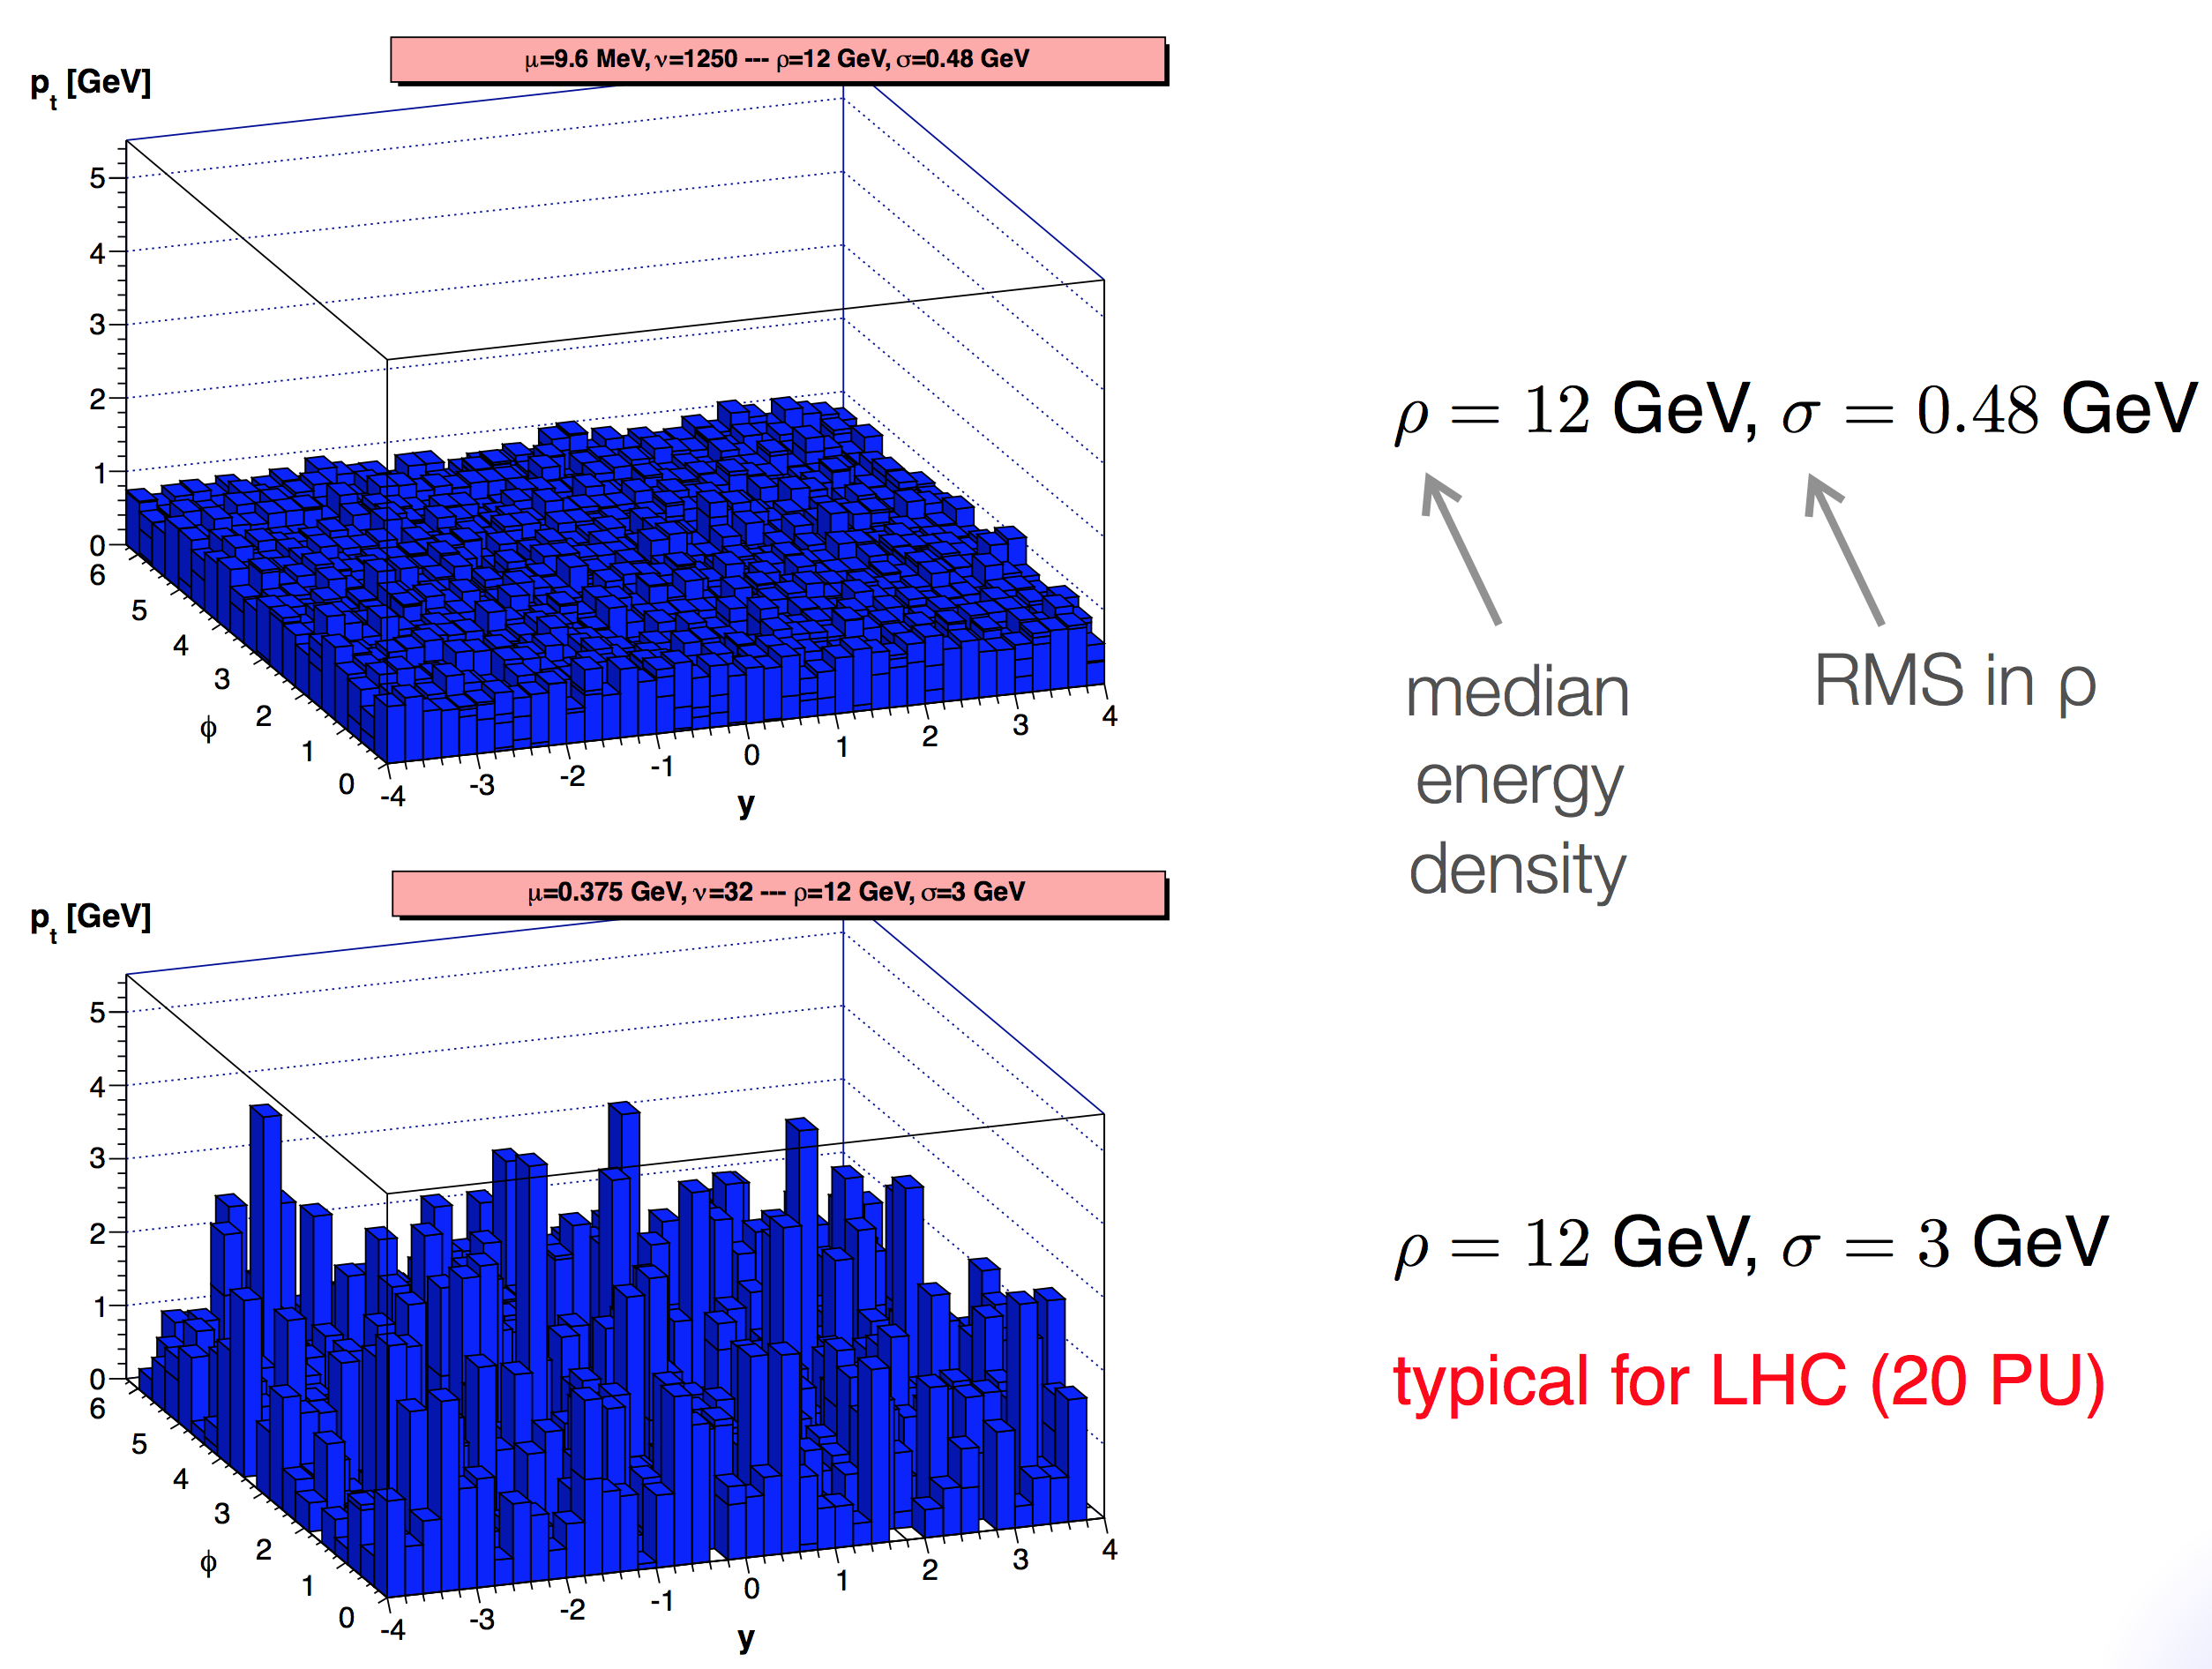
\includegraphics[width=0.85\textwidth]{images/pileup_mitigation/pileup_lumpy.png}
\end{frame}

\begin{frame}[t]\frametitle{PileUp Per Particle Identification (PUPPI)}
	\vspace*{-0.35cm}
    \begin{block}{}
	    \vbox to .88\vsize{
    	\begin{itemize}
    		\item What if we correct for pileup at the particle level?
    		\begin{itemize}
    			\item We already do this for charged particles...
    			\item Can we do it for neutrals too?
    		\end{itemize}
    		\item Inherently local corrections
    		\item If we can, then we don’t have to have different pileup mitigation methods for different objects
    		\begin{itemize}
    			\item jets, MET, leptons/photons
    		\end{itemize}
    		\item \textbf{Idea:} use our knowledge of QCD and the charged information to tell us if a particle is pileup-like or coming from a high $p_{T}$ QCD shower. Assign a weight for every neutral if it’s from pileup or not.
    	\end{itemize}
    	}
    \end{block}
    \begin{textblock}{0.15}(0.843,0.07)
    	
\includegraphics[width=\textwidth]{images/pileup_mitigation/PUPPI_logo.png}
    \end{textblock}
\end{frame}

\begin{frame}[t]\frametitle{What do we know about pileup?}
	\vspace*{-0.35cm}
	\begin{block}{}
		\vbox to .5\vsize{
		Well, many things, but let’s start with some simple properties:\\
		\begin{enumerate}
			\item Due to parton showering, a particle from a \textbf{hard physics process}\\is likely to be near other particles from the same parent process (small $\Delta R$), also higher $p_{T}$
			\item We expect pileup particles to have no shower-like structure and to be uncorrelated with particles from the leading vertex and so only to be spatially near by chance, also lower $p_{T}$
		\end{enumerate}
		\vspace*{-0.65cm}
		}
	\end{block}
	\vspace*{-0.15cm}
	\begin{center}
		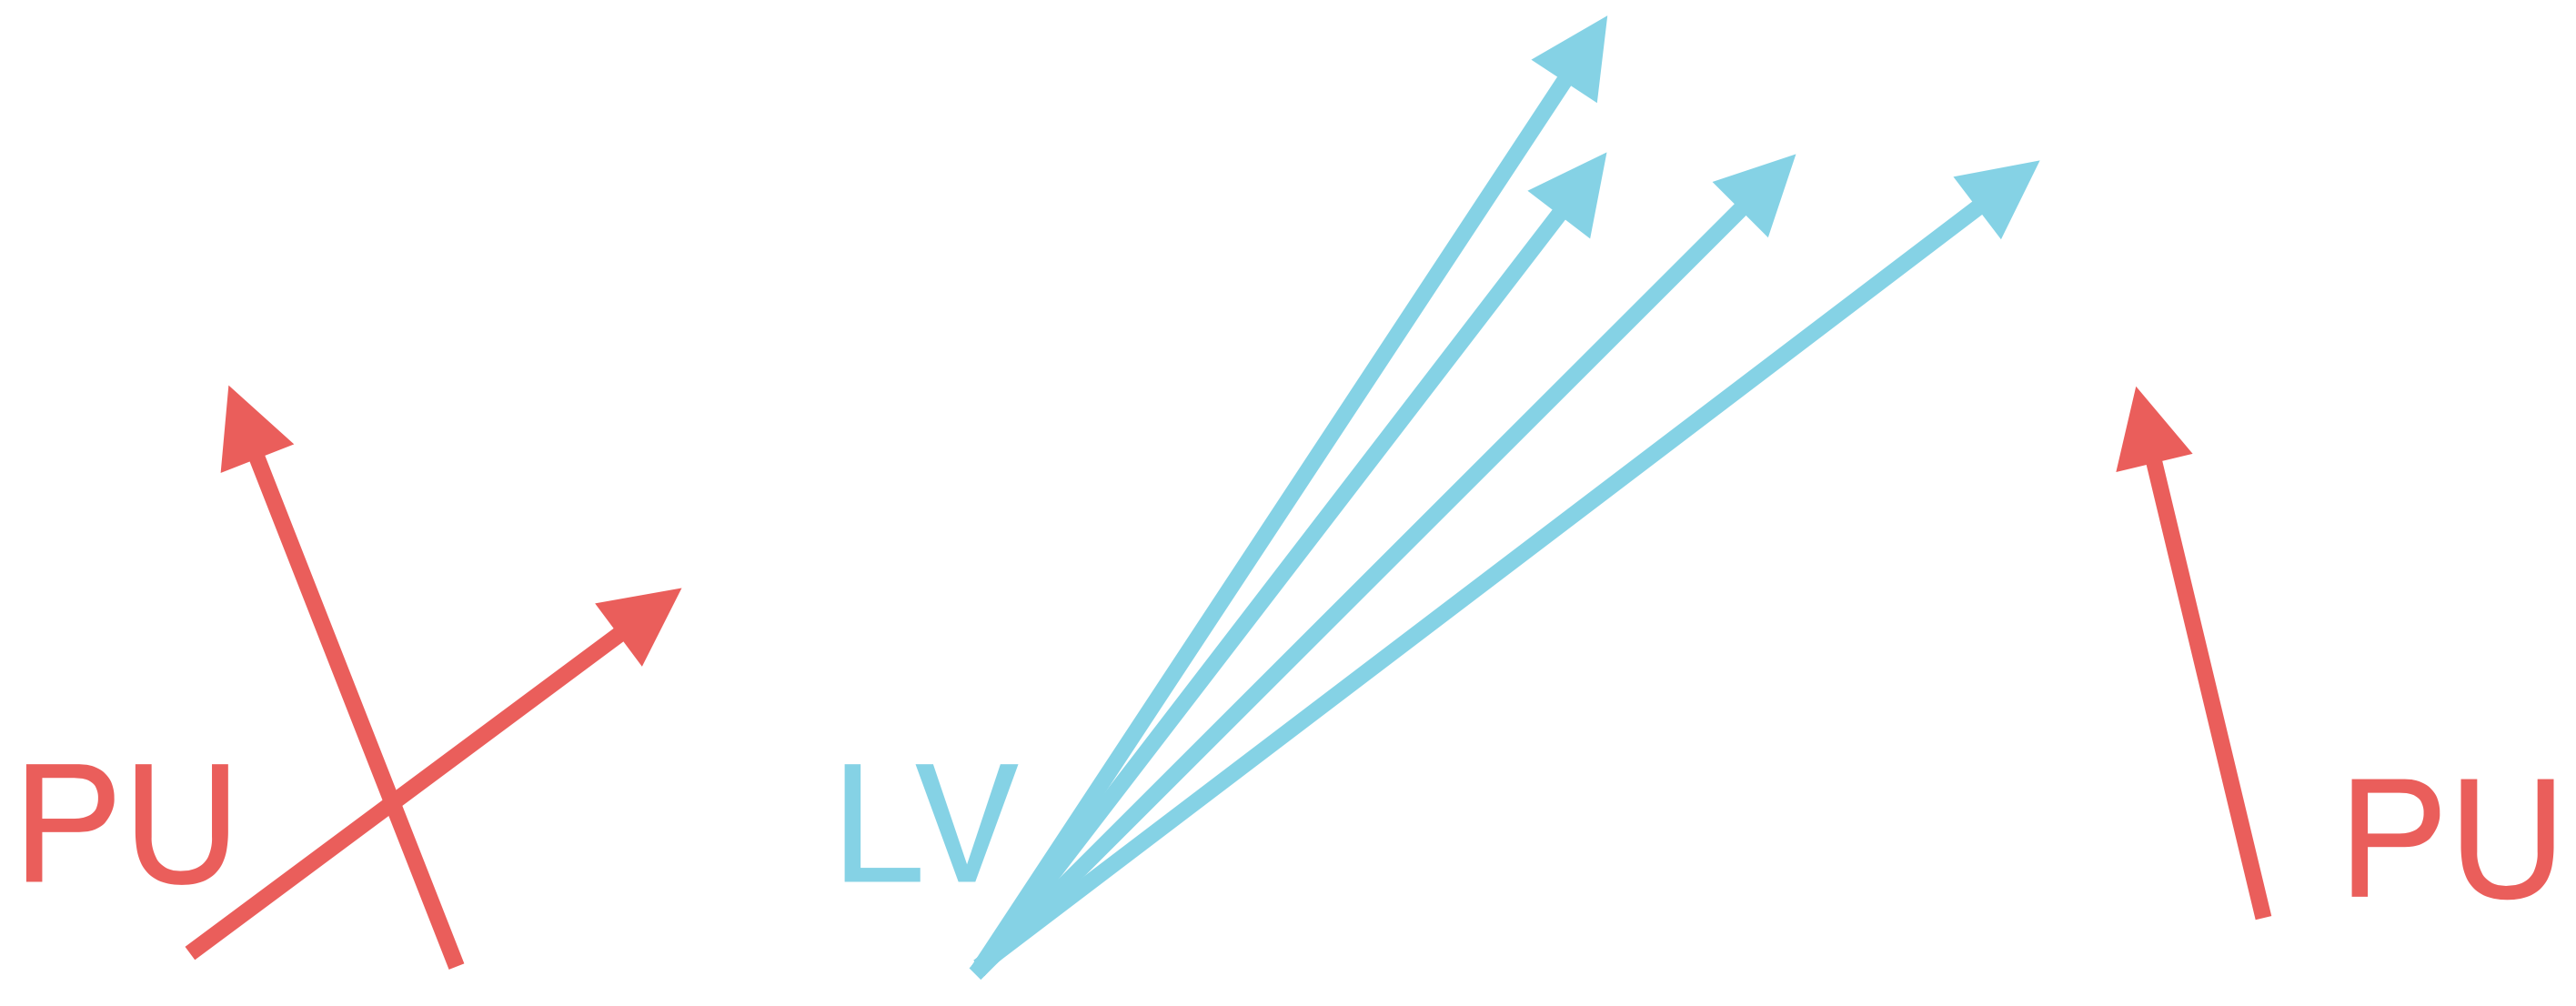
\includegraphics[width=0.67\textwidth]{images/pileup_mitigation/LVvsPU.png}
	\end{center}
    \begin{textblock}{0.15}(0.843,0.07)
    	
\includegraphics[width=\textwidth]{images/pileup_mitigation/PUPPI_logo.png}
    \end{textblock}
\end{frame}

{
\setbeamercolor{background canvas}{bg=}
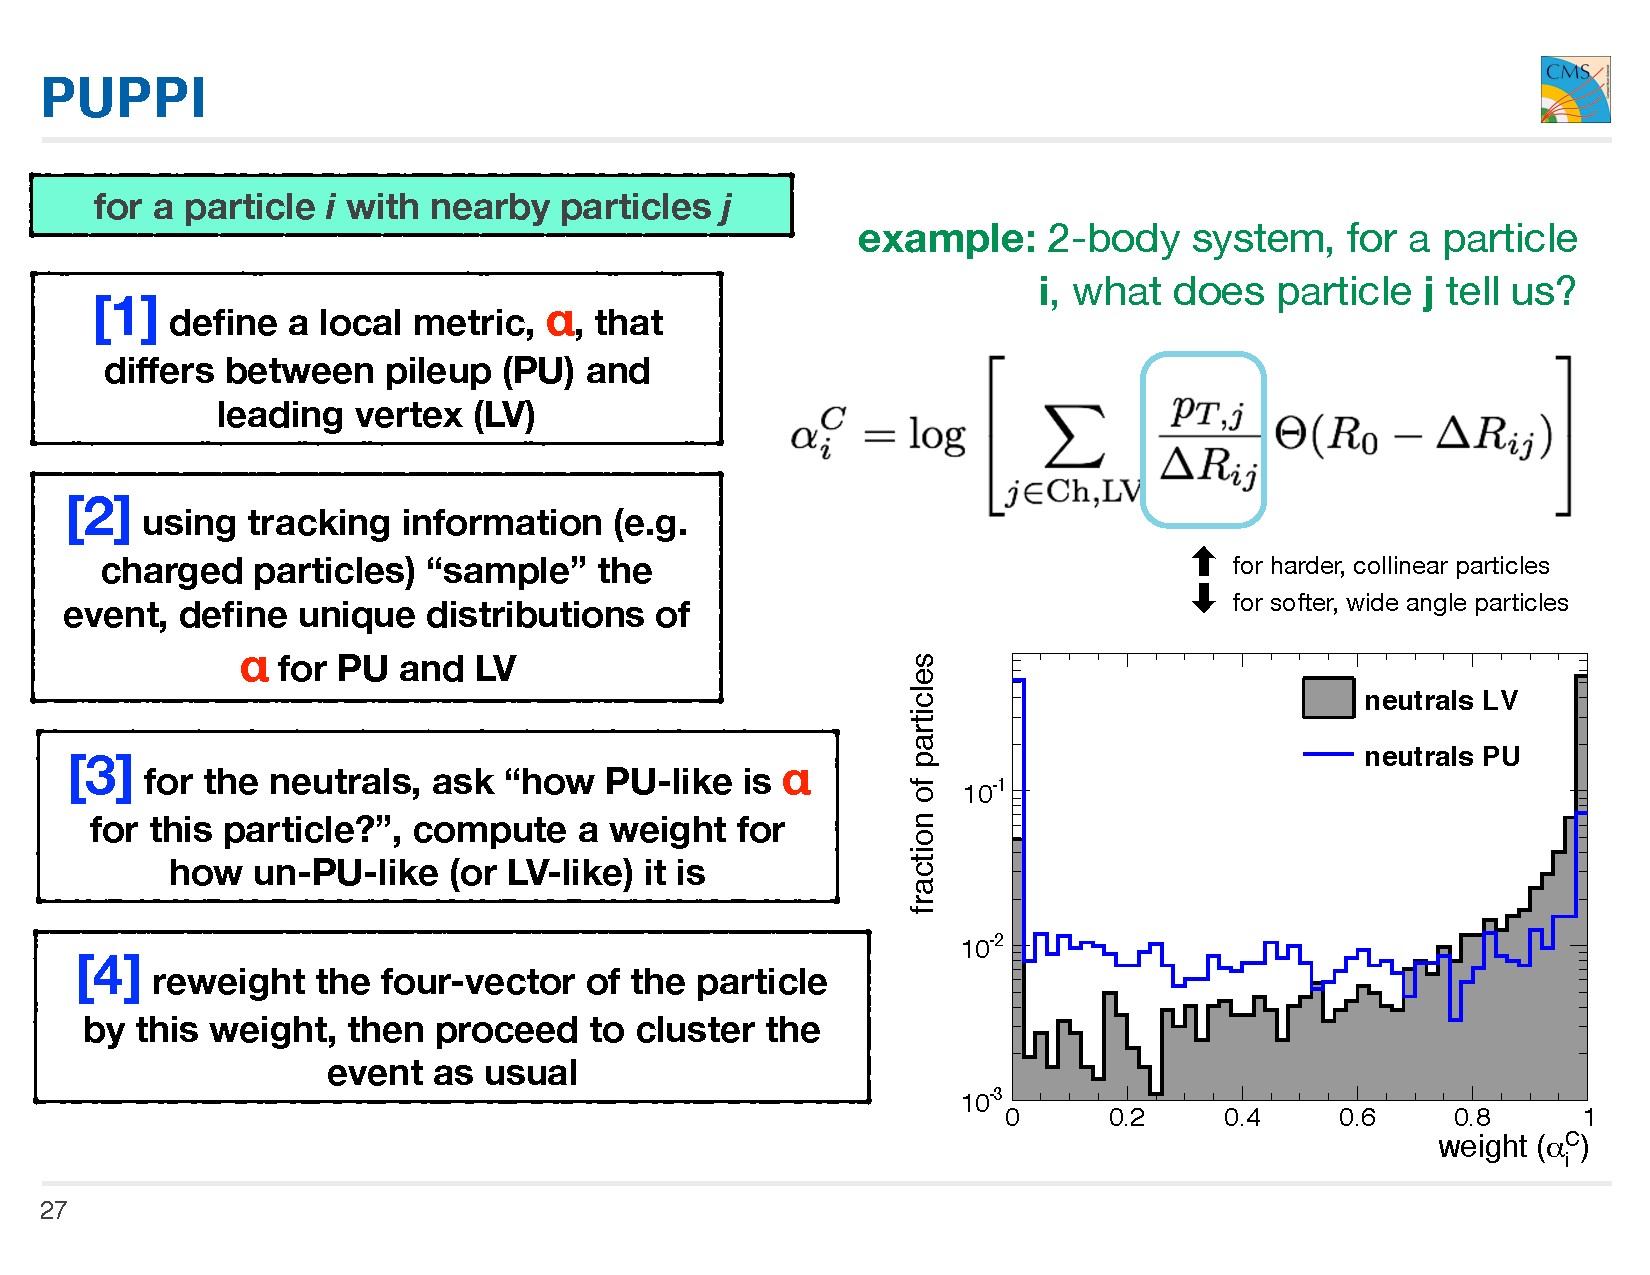
\includepdf[pages=1-3]{images/pileup_mitigation/puppi_explanation.pdf}
}

\addtocounter{framenumber}{3}

\begin{frame}[t]\frametitle{PUPPI}
	\begin{textblock}{0.48}(0.02,0.12)
		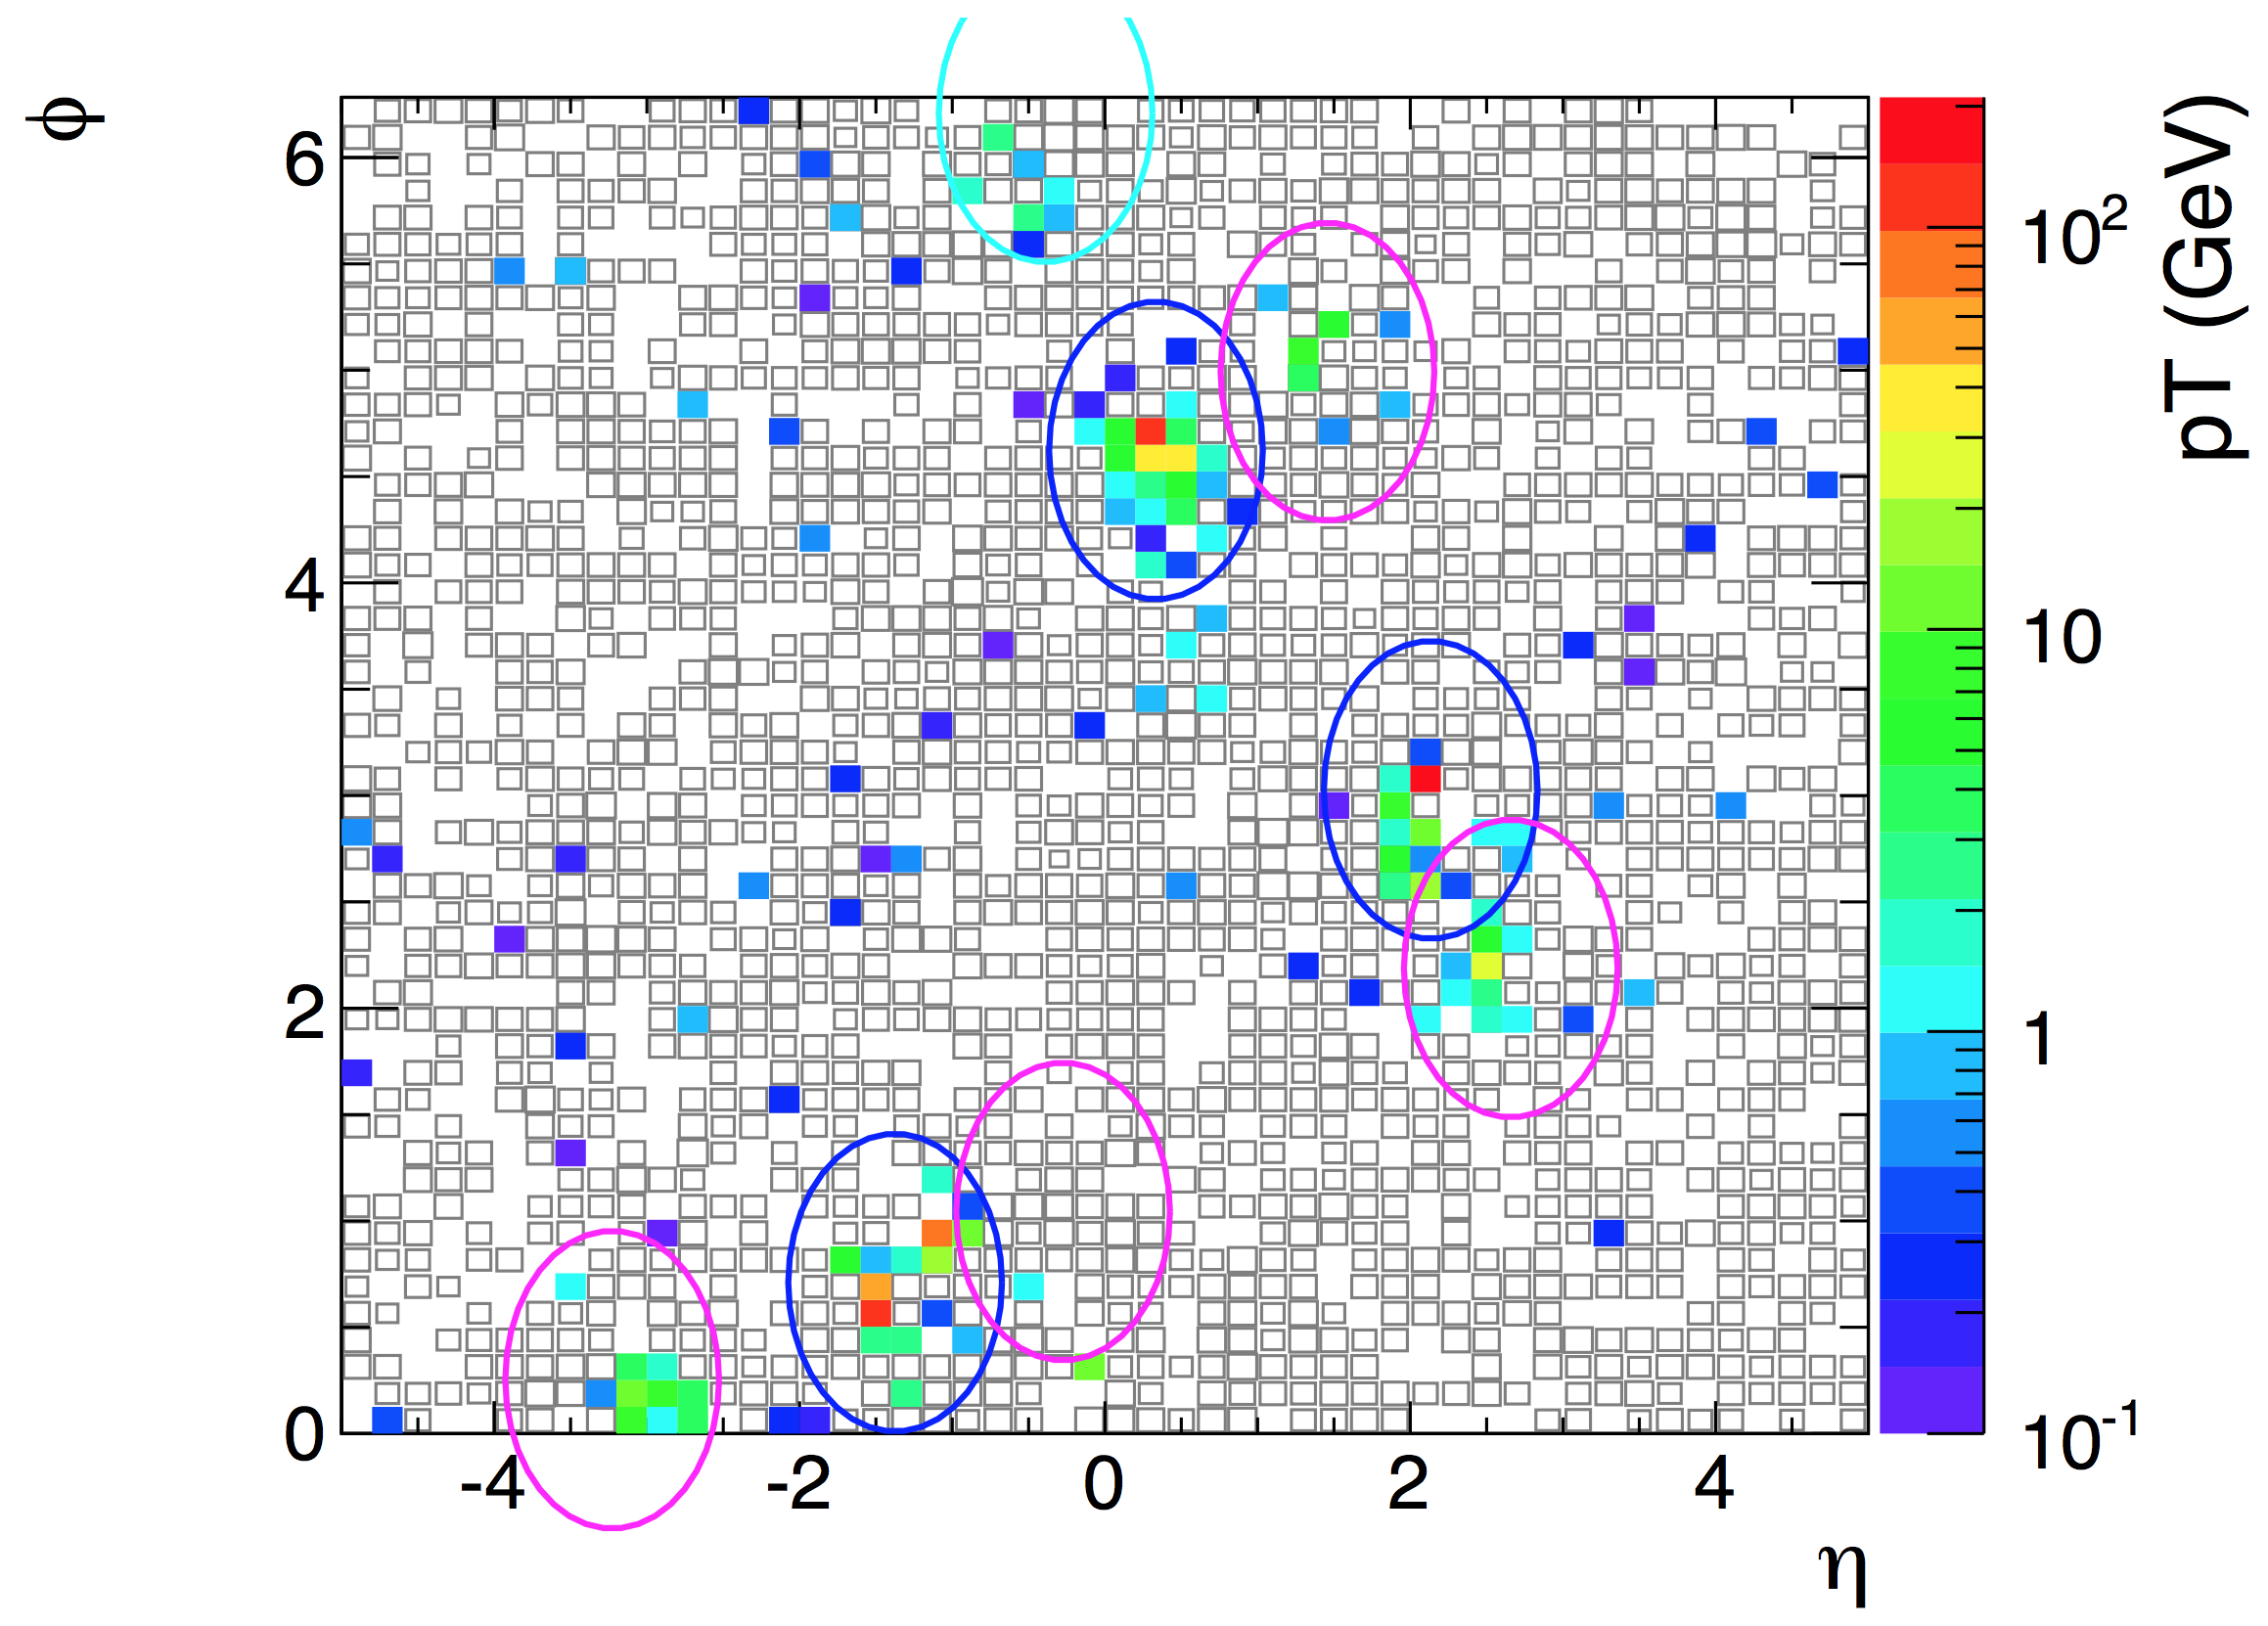
\includegraphics[width=\textwidth]{images/pileup_mitigation/LHC_event_particle_level_pileup.png}
	\end{textblock}
	\begin{textblock}{0.48}(0.51,0.48)
		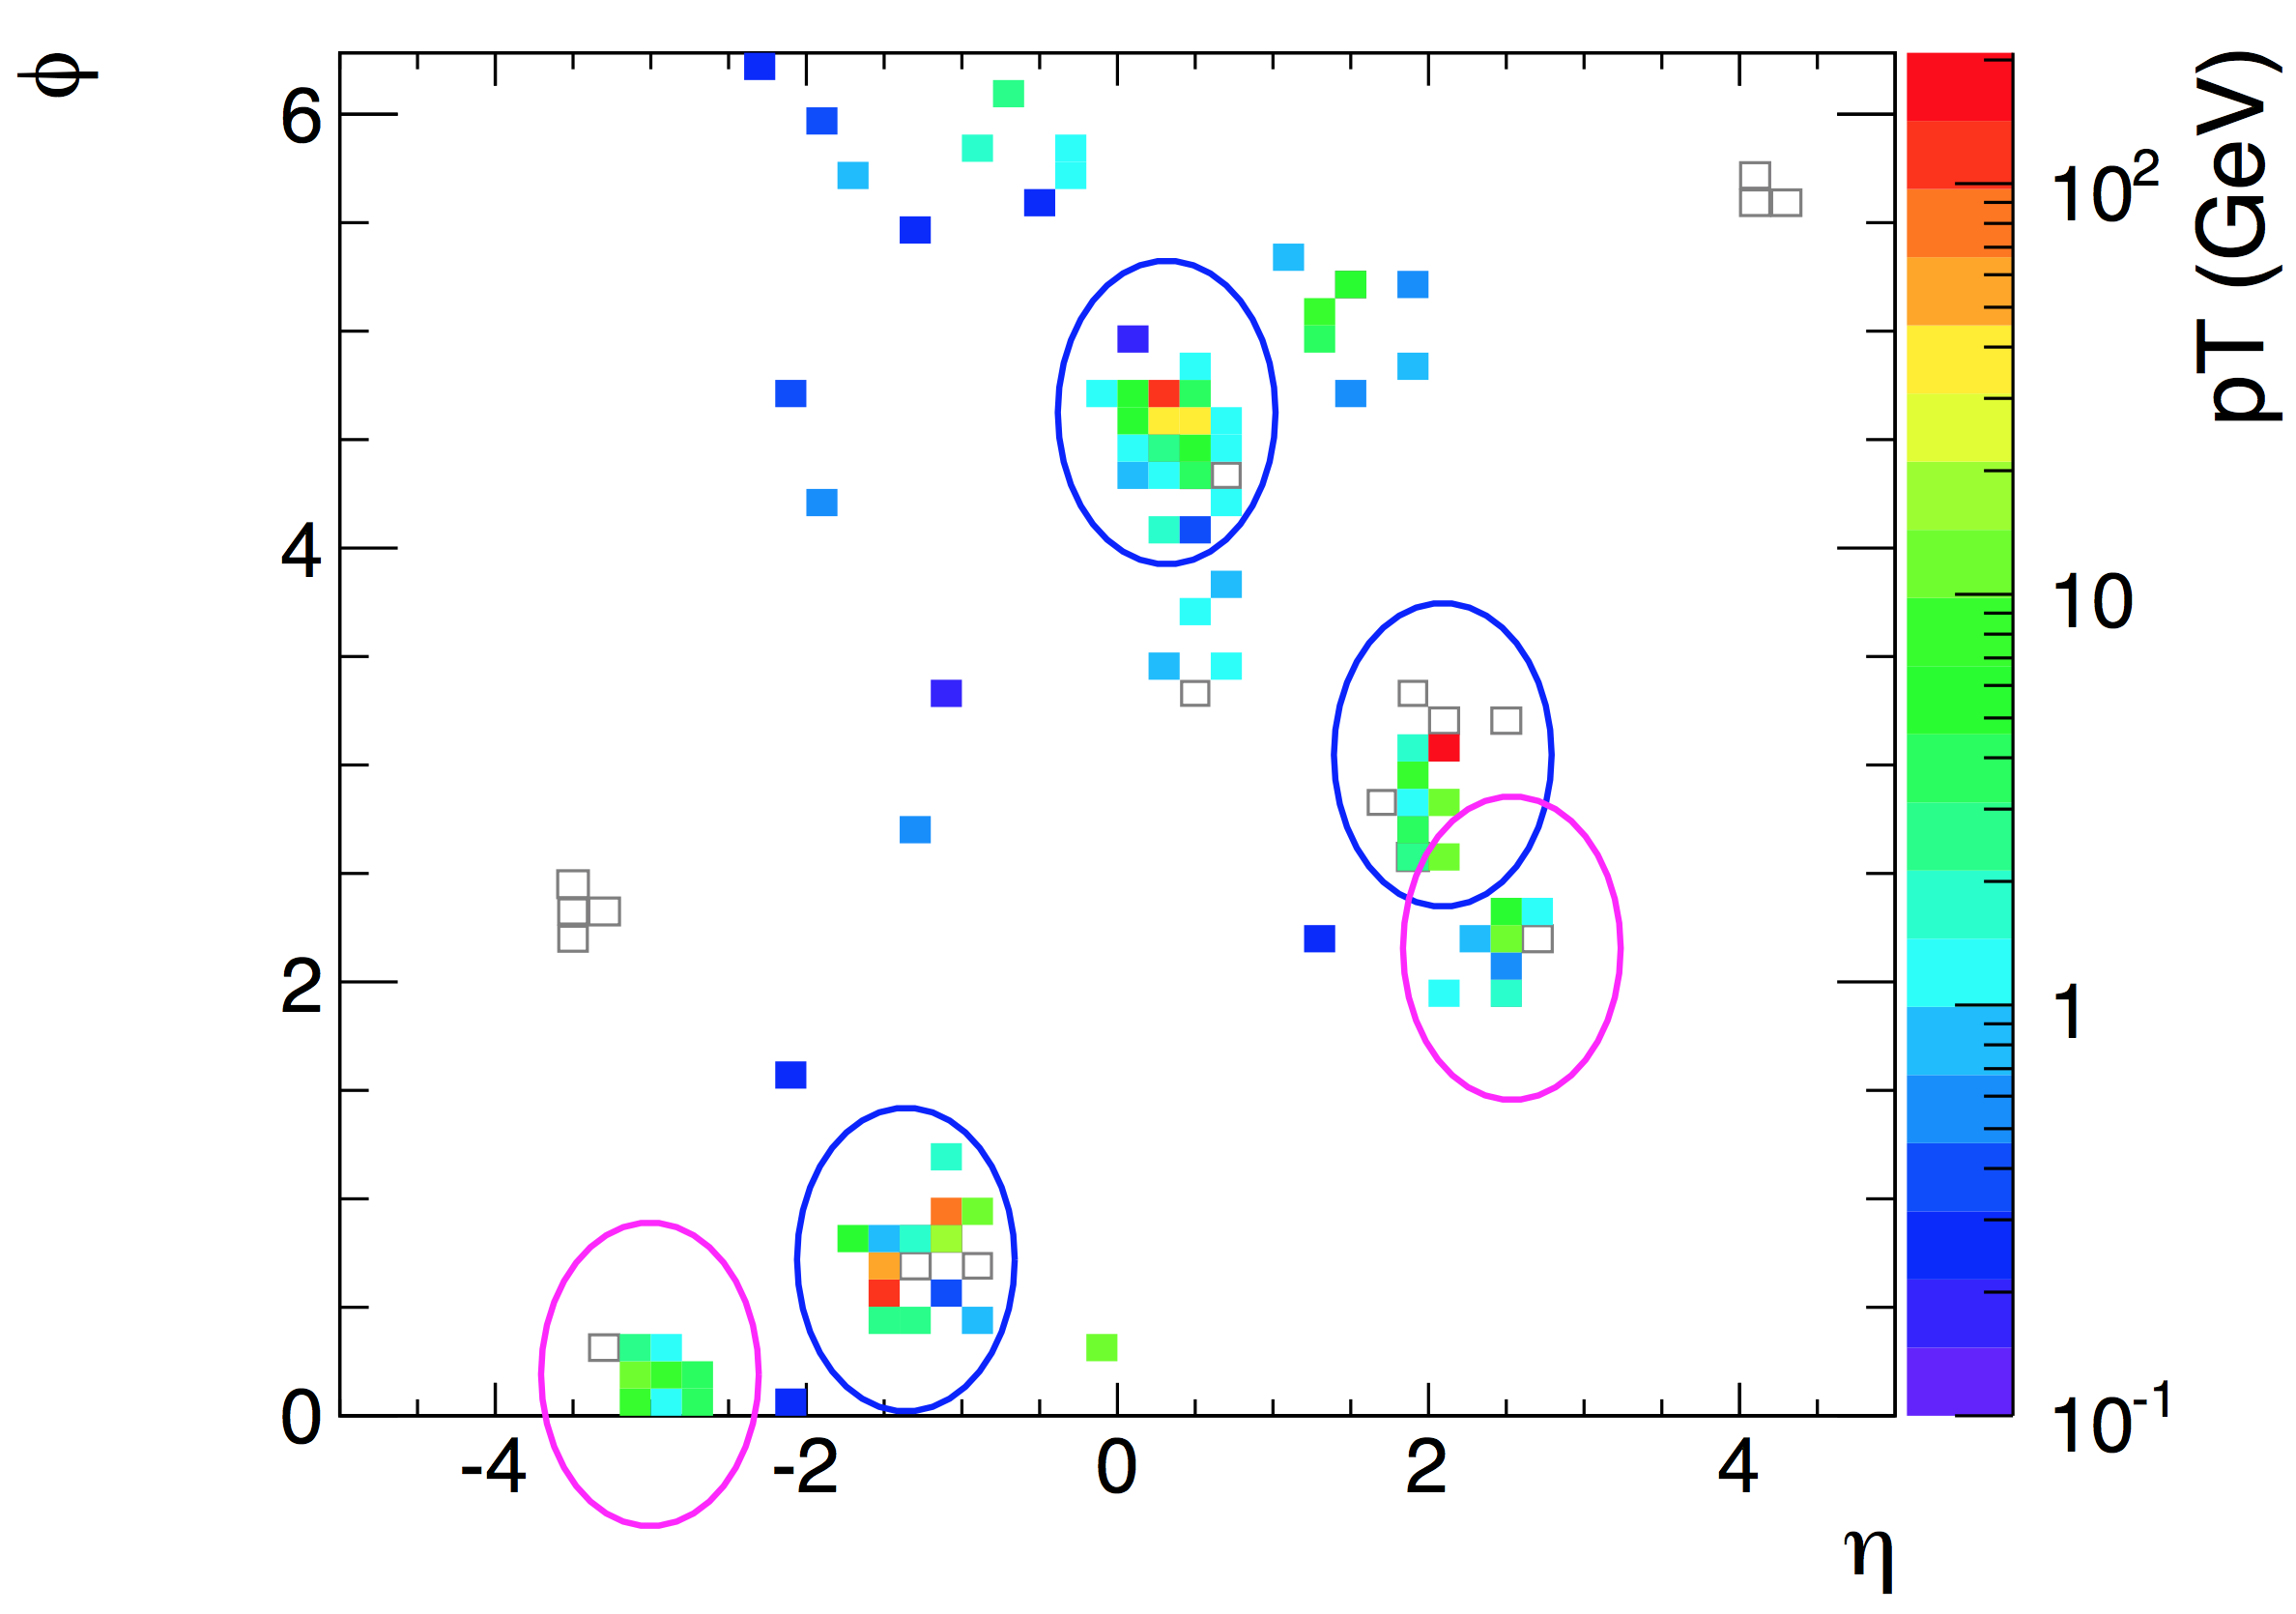
\includegraphics[width=\textwidth]{images/pileup_mitigation/LHC_event_particle_level_puppi.png}
	\end{textblock}
	\begin{textblock}{0.5}(0.02,0.55)
		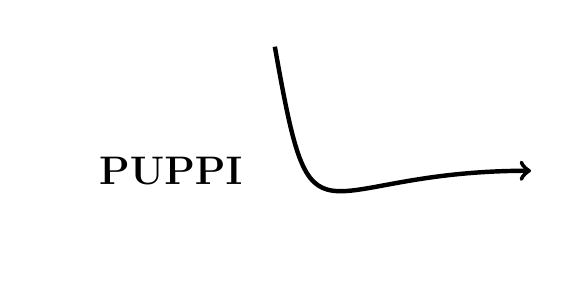
\begin{tikzpicture}
			\node(O) at (0.0,0.0) {};
			\node(A) at (3.0,0.0) {};
			\node(B) at (6.4,-1.7) {};
			\node(pnode) at (1.7,-1.7) {\textbf{\Large PUPPI}};
			\draw[->,ultra thick] (A) to [out=280,in=180,looseness=2] (B);
		\end{tikzpicture}
	\end{textblock}
    \begin{textblock}{0.15}(0.843,0.07)
    	
\includegraphics[width=\textwidth]{images/pileup_mitigation/PUPPI_logo.png}
    \end{textblock}
\end{frame}